\documentclass{report}

\usepackage{ressources/packages/miseEnPage}
\usepackage{ressources/vocabulaire/vocabulaire}

\pdfminorversion=4
\usepackage[francais]{babel}
\usepackage[utf8]{inputenc}
\usepackage[T1]{fontenc}
\usepackage{graphicx}
\usepackage{fancyhdr}
\usepackage{pdfpages}
\usepackage{float}
\usepackage{diagbox}
\usepackage[urlcolor=blue, linkcolor=black,linktoc=all, colorlinks=true]{hyperref}
\usepackage[left=2.5cm, right=2.5cm, top=2.5cm, bottom=2.5cm, headheight=15pt]{geometry}
\usepackage[final]{pdfpages}
\usepackage{helvet}
\usepackage{lscape}
\usepackage{wasysym}
\usepackage[multidot]{grffile}

\renewcommand{\familydefault}{\sfdefault}

\makeatletter
\def\@makechapterhead#1{% chapter
  \vspace*{5\p@}
  {
    \parindent \z@ \raggedright \normalfont
    \ifnum \c@secnumdepth >\m@ne
    \huge\bfseries \@chapapp\space \thechapter
    \par\nobreak
    \vskip 5\p@
    \fi
    \interlinepenalty\@M
    \Huge \bfseries #1\par\nobreak
    \vskip 10\p@
    \thispagestyle{fancy}% Permet d'ajouter l'entête de pied de page
  }
}

\def\@schapter#1{
  \if@twocolumn
  \@topnewpage[\@makeschapterhead{#1}]
  \else
  \@makeschapterhead{#1}
  \@afterheading
  \fi
}

\def\@makeschapterhead#1{% chapter*
  \vspace*{5\p@}
  {
    \parindent \z@ \raggedright
    \normalfont
    \interlinepenalty\@M
    \Huge \bfseries  #1\par\nobreak
    \vskip 10\p@
    \thispagestyle{fancy} % Permet d'ajouter l'entête de pied de page
  }
}
\makeatother


\usepackage[utf8]{inputenc}
\usepackage[T1]{fontenc}
\usepackage[francais]{babel}
\usepackage{graphicx, titlesec}

\begin{document}
\lstset{ %
  backgroundcolor=\color{white},   % choose the background color; you must add \usepackage{color} or \usepackage{xcolor}
  basicstyle=\footnotesize,        % the size of the fonts that are used for the code
  breakatwhitespace=false,         % sets if automatic breaks should only happen at whitespace
  breaklines=true,                 % sets automatic line breaking
  captionpos=b,                    % sets the caption-position to bottom
  commentstyle=\color{mygreen},    % comment style
  deletekeywords={...},            % if you want to delete keywords from the given language
  escapeinside={\%*}{*)},          % if you want to add LaTeX within your code
  extendedchars=true,              % lets you use non-ASCII characters; for 8-bits encodings only, does not work with UTF-8
  frame=single,                    % adds a frame around the code
  keepspaces=true,                 % keeps spaces in text, useful for keeping indentation of code (possibly needs columns=flexible)
  keywordstyle=\color{blue},       % keyword style
  language=C++,                    % the language of the code
  morekeywords={*,...},            % if you want to add more keywords to the set
  numbers=left,                    % where to put the line-numbers; possible values are (none, left, right)
  numbersep=5pt,                   % how far the line-numbers are from the code
  numberstyle=\tiny\color{mygray}, % the style that is used for the line-numbers
  rulecolor=\color{black},         % if not set, the frame-color may be changed on line-breaks within not-black text (e.g. comments (green here))
  showspaces=false,                % show spaces everywhere adding particular underscores; it overrides 'showstringspaces'
  showstringspaces=false,          % underline spaces within strings only
  showtabs=false,                  % show tabs within strings adding particular underscores
  stepnumber=2,                    % the step between two line-numbers. If it's 1, each line will be numbered
  stringstyle=\color{mymauve},     % string literal style
  tabsize=2,                       % sets default tabsize to 2 spaces
  title=\lstname                   % show the filename of files included with \lstinputlisting; also try caption instead of title
} 

\couverture{}
\pagestyle{pageNormale}

\setcounter{page}{1}
\tableofcontents{}
\chapter{Introduction et problématique}
Notre programme sera une plateforme permettant la gestion de portefeuille. Pour cela, nous offrirons la possibilité à l’utilisateur pour chaque actif disponible divers outils d’analyse technique. A partir de cela, nous lui fournirons un conseil concernant l’actif sélectionné (signal de vente, signal d’achat, …). \\ \\
	Nous lui proposerons également une analyse plus pointue qui lui permettra de regarder le comportement de ses actifs en tant que portefeuille par exemple avec la méthode de Black-Scholes ou Markowitz. \\ \\
	La finalité du projet serait de réaliser un jeu en réseau qui permettrait à chaque joueur de créer son portefeuille, de voir son évolution et de la comparer aux autres joueurs : le gagnant sera le joueur le plus riche (ou le moins pauvre). 


\chapter{Besoin et exigences}
Notre projet va donc se découper en trois phases principales : 
\begin{itemize}
\item La première consistera à récupérer les données des cours et les stocker par l’intermédiaire d’une base de données.
\item La deuxième étape sera le traitement de ces données (outils d’analyse technique).
\item Enfin, nous afficherons à l’utilisateur un tableau de bord. 
\end{itemize}

\section{Base de données}
Gestion des différents cours des actifs (Nom, valeur à l’ouverture, à la clôture, la plus haute et la plus basse pendant la séance). \\ \\ 
Deux options pour la récupération des données : soit on les stocke dans une base de donnée statique, c’est-à-dire, nous aurons récupéré les cours pour une certaine durée. Nous placerons le début du jeu dans le passé, de manière à pouvoir constater les gains ou pertes du joueur. La deuxième méthode pour gérer nos données, consisterait à actualiser notre base de données à la demande du joueur en allant chercher les données sur un serveur web. 

\section{Gestion des actifs}
Pour chaque actif nous proposerons une analyse des divers cours que nous aurons dans notre base de données. Pour cela nous utiliserons des outils d’analyse technique. \\ \\
A la fin de l’analyse, nous proposerons un avis sur l’actif. 

\section{Tableau de bord}
Chaque utilisateur aura la possibilité de consulter l’ensemble de son portefeuille. Pour cela un descriptif lui sera affiché avec les fonctionnalités suivantes : détails (composition du portefeuille, liste des actifs), performance et la répartition par titres. \\ \\
Ensuite pour chaque action, il sera possible de visualiser la valeur du cours, sa variation et son volume, un graphique et plusieurs possibilités d’indicateurs. 
\chapter{Modèle de la plateforme}

\section{Cas d'utilisation}
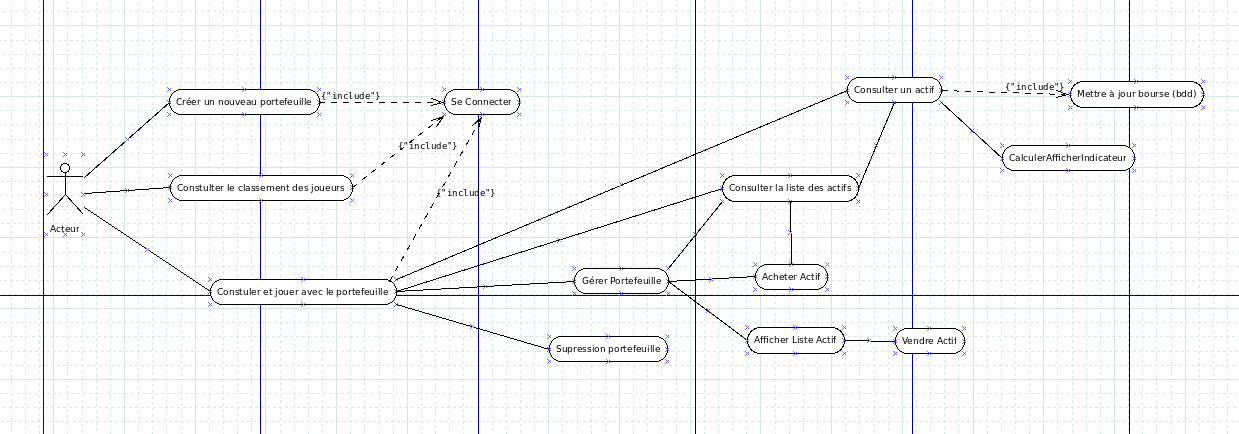
\includegraphics[width=\textwidth,height=\textheight,keepaspectratio]{../graph/CasDutilisationGeneral.png}
\\
Un joueur peut : créer un nouveau portefeuille, consulter l'état du jeu (i.e. le classement des joueurs) ou encore consulter et jouer avec son portefeuille, sous réserve qu'il se soit connecté au préalable. \\ \\
Lorsqu'il choisit de consulter et jouer avec son portefeuille, quatre options s'offrent à lui : il peut consulter un actif précis, consulter la liste des actifs côtés s'il ne sait pas exactement ce qu'il cherche, gérer son portefeuille et jouer, ou encore supprimer son portefeuille afin de stopper la partie. \\ \\
Si le joueur consulte un actif, la bourse sera mise à jour avant qu'il ne puisse éventuellement récupérer un indicateur technique sur ce titre.\\ \\
Si le joueur consulte la liste des actifs, il pourra alors en sélectionner un et se retrouvera dans le cas précédent. \\ \\
Si le joueur choisit de gérer son portefeuille, il peut consulter la liste des actifs de la bourse (et se retrouvera dans la situation précédente), il peut aussi acheter un actif en parcourant la bourse (liste des actifs), et sa dernière possibilité consiste en la consultation des actifs présents dans son portefeuille avant de pouvoir, s'il le souhaite, en vendre une partie.

\section{Diagramme de séquence}
\subsection{Création d'un compte}
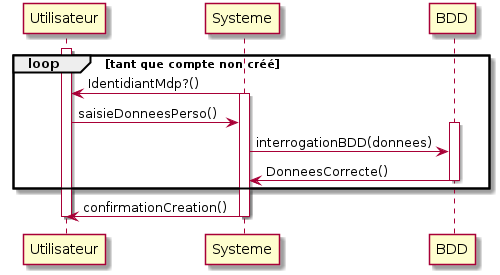
\includegraphics[scale=0.5]{../graph/DiagrammeSequenceCreationCompte.png} \\

\subsection{Authentification}
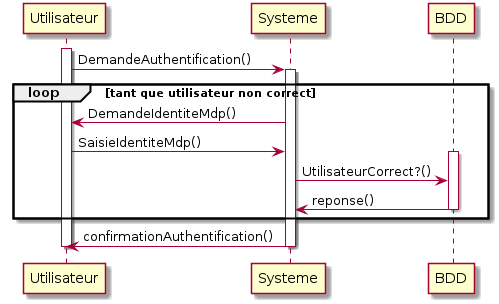
\includegraphics[scale=0.5]{../graph/DiagrammeSequenceAuthentification.png} \\

\subsection{Création d'un nouveau portefeuille}
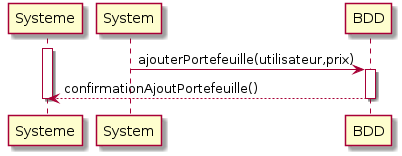
\includegraphics[scale=0.5]{../graph/DiagrammeSequenceCreationPortefeuille.png} \\

\subsection{Consultation du classement des joueurs}
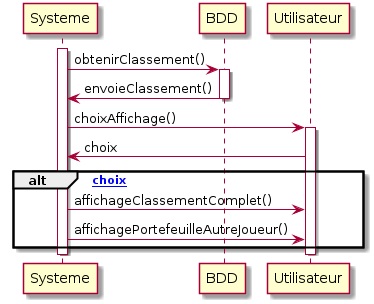
\includegraphics[scale=0.5]{../graph/DiagrammeSequenceConsulterClassement.png} \\

\subsection{Consultation et jeu avec le portefeuille}
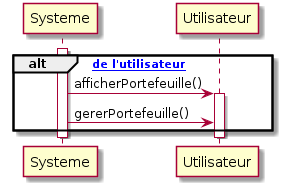
\includegraphics[scale=0.5]{../graph/DiagrammeSequenceConsulterGererPortefeuille.png} \\

\subsection{Consultation d'un actif}
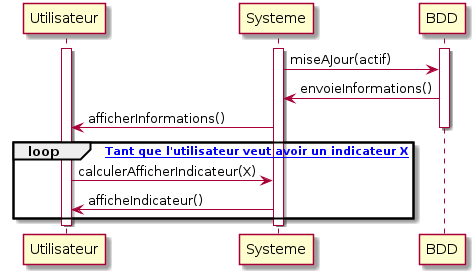
\includegraphics[scale=0.5]{../graph/DiagrammeSequenceConsulterActif.png} \\

\subsection{Affichage d'un indicateur}
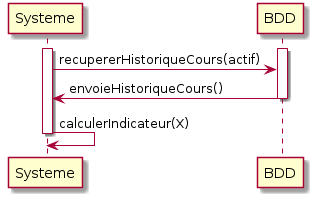
\includegraphics[scale=0.5]{../graph/DiagrammeSequenceCalculerIndicateur.png} \\

\subsection{Consultation de la liste des actifs}
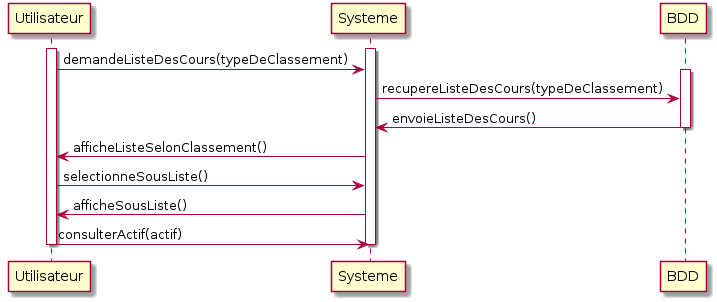
\includegraphics[scale=0.5]{../graph/DiagrammeSequenceConsulterListeActifs.png} \\

\subsection{Gestion du portefeuille}
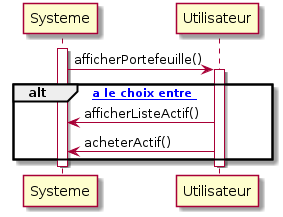
\includegraphics[scale=0.5]{../graph/DiagrammeSequenceGererPortefeuille.png} \\

\subsection{Achat d'un actif}
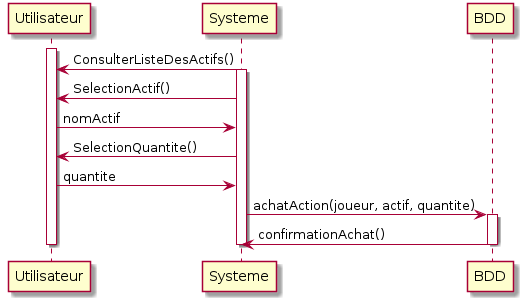
\includegraphics[scale=0.5]{../graph/DiagrammeSequenceAcheterActif.png} \\

\subsection{Affichage de la liste des actifs du portefeuille}
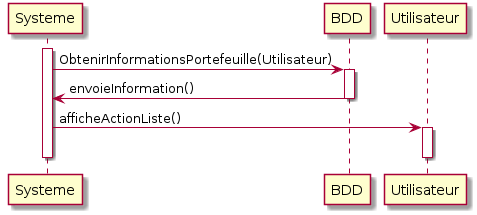
\includegraphics[scale=0.5]{../graph/DiagrammeSequenceAfficherListeAction.png} \\

\subsection{Vente d'un actif}
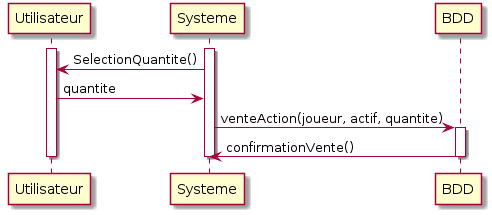
\includegraphics[scale=0.5]{../graph/DiagrammeSequenceVendreActif.png} \\

\subsection{Suppression du portefeuille}
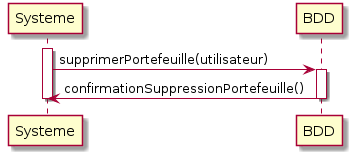
\includegraphics[scale=0.5]{../graph/DiagrammeSequenceSuppressionPortefeuille.png} \\
\chapter{Etude de la base de données}

Nous avons réalisé un modèle entités/associations afin de structurer notre base de données et d'en décrire les tables : \\ \\
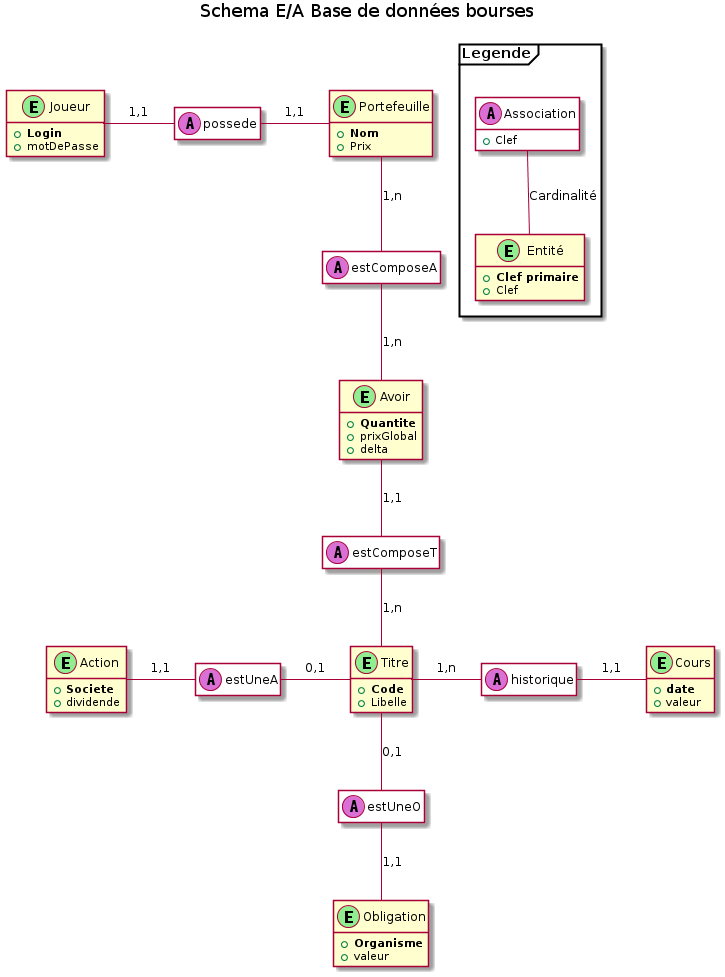
\includegraphics[scale=0.5]{../graph/DiagrammeEntiteAssociation.png} \\
\chapter{Différentes versions envisagées}
Pour réaliser ce projet, nous avons choisi de nous fixer divers objectifs à atteindre. Chacun de ces objectifs correspond à une nouvelle qui sera pour la première une version très simplifiée du projet final à laquelle nous ajouterons les différents éléments au fur et à mesure. \\ 
\section{Version 1}
Dans la première version, le joueur aura la possibilité de s'ajouter à la liste des joueurs, d'ajouter lui même les actions qui constitueront la bourse, d'acheter ou de vendre une action et de voir le contenu de portefeuille. \\ \\
Cette première version nous permettra d'avoir la base de notre projet. 

\section{Version 2}
Dans la deuxième version, nous allons ajouter la dimension base de données à notre projet. C'est-à-dire, que toutes les données qui seront ajoutées au fur et à mesure du jeu ne seront pas perdus comme dans la version précédente quand le jeu se fermera. \\ \\
Ensuite, le joueur n'aura plus la possibilité de choisir les actions et leur valeur lui-même mais il y aura une table qui regroupera les différentes actions qui sont possibles pour le joueur. Nous pourrons ainsi stocker l'historique de chacun des cours également (nous nous contenterons dans un premier temps des actions du CAC 40). 

\section{Version 3}
Dans cette version, nous allons rajouter le téléchargement des cours via l'API Yahoo. A chaque lancement du jeu, nous mettrons à jour la base de données depuis la dernière connexion pour compléter les données manquantes. Nous aurons ainsi un historique complet pour les cours de nos actions. 

\section{Version 4}
Nous allons pour ce nouveau objectif rajouter le tracé des cours. Le joueur pourra avoir une représentation graphique de l'évolution des cours depuis l'historique que nous trouverons dans la base de données remplies précédemment. 

\section{Version 5}
Nous choisirons plusieurs indicateurs techniques que nous mettrons à la disponibilité de chaque joueur. Nous essaierons de lui livrer un conseil à partir de chacun de nos indicateurs (signal de vente, signal d'achat etc). 

\section{Version 6}
Dans cette partie, nous améliorerons la qualité des informations fournies au joueur. Nous  
allons essayer de lui proposer une vision de son portefeuille plus détaillés avec un graphique représentant l'évolution de la valeur de son portefeuille, plus de possibilités en terme d'actions : en essayant d'en augmenter le nombre, de les classifier par secteur, ...


\section{Version 7}
Nous allons pour cette partie développer un véritable mode multijoueur sur un seul ordinateur. Jusqu'à présent le joueur pouvait s'ajouter à la liste des joueurs mais ne devait pas s'identifier par le biais d'un mot de passe ce qui sera mis en place. De plus, il pourra consulter le classement des autres joueurs. 

\section{Version 8}
Dans cette ultime version, nous pourrons nous connecter à notre base de données à distance et ainsi nous pourrons joueur sur plusieurs machines à notre jeu. 
\chapter{Mise en place des méthodes agiles}
Les méthodes agiles sont des groupes de pratiques de projets en développement en informatiques.\\
\\
Elles reposent sur quatre valeurs importantes : \\
\begin{itemize}
\item{L'équipe : il faut une bonne communication entre les membres de l'équipe}
\item{L'application : il faut qu'elle soit fonctionnelle et que la documentation technique soit mise à jour}
\item{La collaboration : le client est impliqué dans le déroulement}
\item{L'acceptation du changement : la planification réalisée est flexible}
\end{itemize} 
~\\
~\\
Les différentes étapes à suivre sont : \\
\begin{itemize}
\item{Le responsable fonctionnel définit et ordonne la production des composants de l'application}
\item{Le projet est structuré en incréments de 1 à 6 semaines suivant les nécessités}
\item{Une réunion initiale organise chaque incrément en définissant les tâches à réaliser}
\item{Chaque jour, courte réunion pour donner à l'équipe une vision globale du projet : avancement, problème et solution}
\item{Reporting mual mis à jour et en temps réel par les membres de l'équipe}
\item{Un incrément est terminé s'il est complet, développé, approuvé, testé et documenté}
\item{Réunion finale pour chaque incrément}
\item{Validation du travail de l'équipe par le responsable fonctionnel}
\end{itemize}

\pageQuatriemeCouverture{}
\end{document}
